\documentclass[10pt, landscape]{article}
\usepackage[scaled=0.92]{helvet}
\usepackage{calc}
\usepackage{multicol}
\usepackage[a4paper,margin=3mm,landscape]{geometry}
\usepackage{amsmath,amsfonts,amssymb}
\usepackage{color,graphicx,overpic}
\usepackage{hyperref}
\usepackage{newtxtext} 
\usepackage{enumitem}
\usepackage[table]{xcolor}
\usepackage{mathtools}
\usepackage{tikz}
\setlist{nosep}
% for including images
\graphicspath{ {./images/} }

\pdfinfo{
  /Title (ST2131.pdf)
  /Creator (TeX)
  /Producer (pdfTeX 1.40.0)
  /Author (Jovyn Tan)
  /Subject (ST2131)
/Keywords (ST2131, nus,cheatsheet,pdf)}

% Turn off header and footer
\pagestyle{empty}

% redefine section commands to use less space
\makeatletter
\renewcommand{\section}{\@startsection{section}{1}{0mm}%
  {-1ex plus -.5ex minus -.2ex}%
  {0.5ex plus .2ex}%x
{\normalfont\large\bfseries}}
\renewcommand{\subsection}{\@startsection{subsection}{2}{0mm}%
  {-1explus -.5ex minus -.2ex}%
  {0.5ex plus .2ex}%
{\normalfont\normalsize\bfseries}}
\renewcommand{\subsubsection}{\@startsection{subsubsection}{3}{0mm}%
  {-1ex plus -.5ex minus -.2ex}%
  {1ex plus .2ex}%
{\normalfont\small\bfseries}}%
\makeatother

\renewcommand{\familydefault}{\sfdefault}
\renewcommand\rmdefault{\sfdefault}
%  makes nested numbering (e.g. 1.1.1, 1.1.2, etc)
\renewcommand{\labelenumii}{\theenumii}
\renewcommand{\theenumii}{\theenumi.\arabic{enumii}.}
\renewcommand\labelitemii{•}
\renewcommand\labelitemiii{•}

\definecolor{mathblue}{cmyk}{1,.72,0,.38}
\everymath\expandafter{\the\everymath \color{mathblue}}

% Don't print section numbers
\setcounter{secnumdepth}{0}

%% adjust spacing for all itemize/enumerate
\setlength{\leftmargini}{0.5cm}
\setlength{\leftmarginii}{0.5cm}
\setlist[itemize,1]{leftmargin=2mm,labelindent=1mm,labelsep=1mm}
\setlist[itemize,2]{leftmargin=4mm,labelindent=1mm,labelsep=1mm}

% adding my commands
% tightcenter
\newenvironment{tightcenter}{%
  \setlength\topsep{0pt}
  \setlength\parskip{0pt}
  \begin{center}
    }{%
  \end{center}
}

% boxed
\newenvironment{tightbox}{%
  \setlength\topsep{0pt}
  \setlength\parskip{0pt}
  \begin{center}
    \begin{tabular}{|@{\hspace{\dimexpr\fboxsep+0.5\arrayrulewidth}}c@{\hspace{\dimexpr\fboxsep+0.5\arrayrulewidth}}|}
      \hline
    }
    {%
    \\ \hline
    \end{tabular}
  \end{center}
}

% fixed width box
\newenvironment{fixedbox}[1][0.7]{
  \setlength\topsep{0pt}
  \setlength\parskip{0pt}
  \begin{center}
    \begin{tabular}{|>{\centering\arraybackslash}m{#1\linewidth}|}
    \hline
  }{
  \\ \hline
  \end{tabular}
  \end{center}
}

% definition of a new term
\usepackage{soul}
\definecolor{paleyellow}{RGB}{251,243,218}
\newcommand{\definition}[2][]{\sethlcolor{paleyellow}\hl{\textbf{#2}} #1  $\rightarrow$}

% important note (attention)
\newcommand{\attention}{{\color{red}\textbf{! }}}


% proofs
\newenvironment{proof}
{%
  \sbox0{\textit{Proof}: }%
  \list{}{\labelwidth\wd0 \leftmargin\wd0 \labelsep 0pt }
\item[\usebox0]}
  {\endlist}


% -----------------------------------------------------------------------

\begin{document}
\raggedright
\footnotesize

% space above/below equation environment 
\setlength{\abovedisplayskip}{1pt}
\setlength{\belowdisplayskip}{1pt}

\begin{multicols*}{3}
  % multicol parameters
  \setlength{\columnseprule}{0.25pt}

  \begin{center}
    \fbox{%
      \parbox{0.8\linewidth}{\centering \textcolor{black}{
          {\Large\textbf{ST2131}}
        \\ \normalsize{AY21/22 SEM 2}}
        \\ {\footnotesize \textcolor{gray}{github/jovyntls}}
      }%
    }
  \end{center}

  \section{01. COMBINATORIAL ANALYSIS}

  \textbf{tricky} - E18, E20-22, E23, E26

  \subsection{The Basic Principle of Counting}

  \begin{itemize}
    \item \definition{combinatorial analysis} the mathematical theory of counting
    \item \definition{basic principle of counting} Suppose that two experiments are performed. 
      If exp1 can result in any one of $m$ possible outcomes and if, for each outcome of exp1, there are $n$ possible outcomes of exp2, 
      then together there are $mn$ possible outcomes of the two experiments.
    \item \definition{generalized basic principle of counting} If $r$ experiments are performed such that the first one may result in any of $n_1$ possible outcomes and if for each of these $n_1$ possible outcomes, and if ..., then there is a total of $n_1 \cdot n_2 \cdot \dots \cdot n_r$ possible outcomes of $r$ experiments.
  \end{itemize}

  \subsection{Permutations}

  \textbf{factorials} - $1! = 0! = 1$

  \textbf{N1} - if we know how to count the number of different ways that an event can occur, we will know the probability of the event.

  \textbf{N2} - there are $n!$ different arrangements for $n$ objects.

  \textbf{N3} - there are $\frac{n!}{n_1!\, n_2!\, \dots n_r!}$ different arrangements of $n$ objects, 
  of which $n_1$ are alike, $n_2$ are alike, ..., $n_r$ are alike.

  \subsection{Combinations}

  \textbf{N4} - $\binom{n}{r} = \frac{n!}{(n-r)!\,r!}$ represents the number of different groups of size $r$ that could be selected from a set of $n$ objects when the order of selection is not considered relevant.

  \textbf{N4b} - $\binom{n}{r} = \binom{n-1}{r-1} + \binom{n-1}{r}, \quad 1 \leq r \leq n$
  \begin{proof}
    If object 1 is chosen $\Rightarrow$ $\binom{n-1}{r-1}$ ways of choosing the remaining objects.
    \\* If object 1 is not chosen $\Rightarrow$ $\binom{n-1}{r}$ ways of choosing the remaining objects.
  \end{proof}

  \textbf{N5} - \textbf{The Binomial Theorem} - \( {\displaystyle{(x+y)^n = \sum^n_{k=0} \binom{n}{k} x^k y^{n-k} }} \) 
  \begin{proof}
    by mathematical induction: $n=1$ is true; expand; sub dummy variable; combine using N4b; combine back to final term
  \end{proof}

  \subsection{Multinomial Coefficients}

  \textbf{N6} - $\binom{n}{n_1, n_2, \dots, n_r} = \frac{n!}{n_1!\, n_2!\, \dots \, n_r!}$  
  represents the number of possible divisions of $n$ distrinct objects 
  into $r$ distinct groups of respective sizes $n_1, n_2, \dots, n_3$, 
  where $n_1 + n_2 + \dots + n_r = n$
  \begin{proof}
    using basic counting principle, 
    \\* $= \binom{n}{n_1} \binom{n-n_1}{n_2} \binom{n-n_1-n_2}{n_3} \dots \binom{n-n_1-n_2-n_{r-1}}{n_r}$
    \\* $= \frac{n!}{(n-n_1)!\,n_1!} \times \frac{(n-n_1)!}{(n-n_1-n_2)!\, n_2!} \times \dots \times \frac{( n-n_1-n_2-\dots -n_{r-1} )}{0!\, n_r!}$
    \\* $= \frac{n!}{n_1!\, n_2! \, \dots \, n_r!}$
  \end{proof}

  \textbf{N7} - \textbf{The Multinomial Theorem}: $(x_1 + x_2 + \dots + x_r)^n$
  \\* $ \quad\quad\quad = \sum\limits_{(n_1, \dots, n_r):n_1 + n_2 + \dots + n_r = n} \frac{n!}{n_1! \, n_2! \, \dots n_r!} x_1^{n_1} x_2^{n_2} \dots x_r^{n_r}$

  \subsection{Number of Integer Solutions of Equations}

  \textbf{N8} - there are $\binom{n-1}{r-1}$ distinct \textit{positive} integer-valued vectors $(x_1, x_2, \dots, x_r)$ satisfying
  $x_1 + x_2 + \dots + x_r = n, \quad x_i > 0, \quad i = 1,2,\dots,r$  
  \\* \attention cannot be directly applied to \textit{N8} as 0 value is not included

  \textbf{N9} - there are $\binom{n+r-1}{r-1}$ distinct  \textit{non-negative} integer-valued vectors $(x_1, x_2, \dots, x_r)$ satisfying $x_1 + x_2 + \dots + x_r = n$ 
  \begin{proof}
    let $y_k = x_k + 1 \Rightarrow y_1 + y_2 + \dots + y_r = n + r$
  \end{proof}


  \section{02. AXIOMS OF PROBABILITY}

  \subsection{Sample Space and Events}
  \begin{itemize}
    \item \definition{sample space} The \textit{set} of all outcomes of an experiment (where outcomes are not predictable with certainty)
    \item \definition{event} Any \textit{subset} of the sample space
    \item \definition[of events $E$ and $F$]{union} $E \cup F$ is the event that contains all outcomes that are either in $E$ or $F$ (or both).
    \item \definition[of events $E$ and $F$]{intersection} $E \cap F$ or $EF$ is the event that contains all outcomes that are both in $E$ and in $F$.
    \item \definition[of $E$]{complement} $E^c$ is the event that contains all outcomes that are \textit{not} in $E$.
    \item \definition{subset} $E \subset F$ is all of the outcomes in $E$ that are also in $F$.
      \begin{itemize}
        \item $E \subset F \land F \subset E \Rightarrow E = F$
      \end{itemize}
  \end{itemize}

  \subsubsection{DeMorgan's Laws}
  $\mathbf{ (\bigcup\limits^n_{i=1} E_i)^c = \bigcap\limits^n_{i=1}E_i^c }$ 
  \begin{proof}
    to show LHS $\subset$ RHS: let $x \in (\bigcup^n_{i=1}E_i)^c$ 
    \\* $\quad\Rightarrow x \notin \bigcup^n_{i=1}E_i \Rightarrow x \notin E_1$ and $x \notin E_2 \dots$ and $x \notin E_n$
    \\* $\quad\Rightarrow x \in E_1^c$  and $x \in E_2^c \dots$ and $x \in E_n^c$
    \\* $\quad\Rightarrow x \in \bigcap^n_{i=1} E_i^c$
    \\* to show RHS $\subset$ LHS: let $x \in \bigcap^n_{i=1} E_i^c$
  \end{proof}

  $\mathbf{ (\bigcap\limits^n_{i=1}E_i)^c = \bigcup\limits^n_{i=1}E_i^c }$ \\
  \begin{proof}
    using the first law of DeMorgan, negate LHS to get RHS
  \end{proof}


  \subsection{Axioms of Probability}

  \subsubsection{definition 1: relative frequency}
  \begin{equation*}
    P(E) = \lim_{n \to \infty} \frac{n(E)}{n} 
  \end{equation*}
  problems with this definition:
  \begin{enumerate}
    \item $\frac{n(E)}{n}$ may not converge when $n \to \infty$ 
    \item $\frac{n(E)}{n}$ may not converge to the same value if the experiment is repeated
  \end{enumerate}

  \subsubsection{definition 2: Axioms}

  Consider an experiment with sample space $S$. 
  For each event $E$ of the sample space $S$, we assume that a number $P(E)$ is definned and satisfies the following 3 axioms:
  \begin{enumerate}
    \item $0 \leq P(E) \leq 1$ 
    \item $P(S) = 1$
    \item For any sequence of mutually exclusive events $E_1, E_2, \dots$ 
      \\* (i.e., events for which $E_iE_j = \emptyset$ when  $i \neq j$),
      \begin{tightcenter}
        $P(\bigcup\limits^\infty_{i=1} E_i) = \sum\limits^\infty_{i=1} P(E_i)$ 
      \end{tightcenter}
  \end{enumerate}
  $P(E)$ is the probability of event $E$.

  \subsection{Simple Propositions}

  \textbf{N1} - $P(\emptyset) = 0$

  \textbf{N2} - $P(\bigcup\limits^n_{i=1} E_i) = \sum\limits^n_{i=1} P(E_i)$ 
  $\quad$ (aka axiom 3 for a finite $n$)

  \textbf{N3} - \textbf{strong law of large numbers} - if an experiment is repeated over and over again, then with probability $1$, 
  the proportion of time during which any specific event $E$ occurs will be equal to $P(E)$.

  \textbf{N6} - the definitions of probability are mathematical definitions. 
  They tell us which set functions can be called \textbf{probability functions}. 
  They do not tell us what value a probability function $P(\cdot)$ assigns to a given event $E$.

  \begin{tightcenter}
    probability function $\iff$ it satisfies the 3 axioms.
  \end{tightcenter}

  \textbf{N7} - $P(E_c) = 1-P(E)$

  \textbf{N8} - if $E \subset F$, then $P(E) \leq P(F)$

  \textbf{N9} - $P(E \cup F) = P(E) + P(F) - P(E \cap F)$

  \textbf{N10} - Inclusion-Exclusion identity where $n=3$
  \begin{align*}
    P(E \cup F \cup G) &= P(E) + P(F) + P(G) \\*
                       &- P(EF) - P(EG) - P(FG) \\*
                       &+ P(EFG)
  \end{align*}

  \textbf{N11} - \textbf{Inclusion-Exclusion identity} - 
  \begin{align*}
    P(E_1 \cup E_2 \cup \dots \cup E_n) &= \sum\limits^n_{i=1} P(E_i) - \sum\limits_{i_1 < i_2} P(E_{i_1} E_{i_2}) + \dots \\
                                        &+ (-1)^{r+1} \sum_{i_1 < i_2 < \dots < i_r} P(E_{i_1} E_{i_2} \dots E_{i_r}) + \dots \\
                                        &+ (-1)^{n+1} P(E_1 E_2 \dots E_n)
  \end{align*}
  \begin{proof}
    Suppose an outcome with probability $\omega$ is in exactly $m$ of the events $E_i$, where $m > 0$. Then
    \\* \textbf{LHS}: the outcome is in $E_1\cup E_2 \cup \dots \cup E_n$ and $\omega$ will be counted once in $P(E_1\cup E_2 \cup \dots \cup E_n)$ 
    \\* \textbf{RHS}: 
    \begin{itemize}
      \item the outcome is in exactly $m$ of the events $E_i$ and $\omega$ will be counted exactly $\binom{m}{1}$ times in $\sum\limits^n_{i=1}P(E_i)$
      \item the outcome is contained in $\binom{m}{2}$ subsets of the type $E_{i_1}E_{i_2}$ 
        and $\omega$ will be counted $\binom{m}{2}$ times in $\sum\limits_{i_1 < i_2} P(E_{i_1} E_{i_2})$ 
      \item $\dots$ and so on 
    \end{itemize}
    hence RHS = $\binom{m}{1}\omega - \binom{m}{2}\omega + \binom{m}{3}\omega - \dots \pm \binom{m}{m}\omega $
    \\ $\quad = \omega \sum\limits^m_{i=0}\binom{m}{i} (-1)^i = $ binomial theorem where $x=-1, y=1$ 
    \\ $\quad = 0 = $ LHS
  \end{proof}
  \begin{proof}[e.g]
    For an outcome with probability $\omega$ and $n=3$
    \begin{itemize}
      \item 
        \begin{proof}[Case 1] $w = P(E_1E_2)$
          \\* LHS = $\omega$
          \\* RHS = ($\omega$ + $\omega$ + 0) - ($\omega$ + 0 + 0) + 0 = $\omega$
        \end{proof}
      \item 
        \begin{proof}[Case 2] $\omega = P(E_1 \cap E_2 \cap E_3)$
          \\* LHS = $\omega$
          \\* RHS = ($\omega$ + $\omega$ + $\omega$) - ($\omega$ + $\omega$ + $\omega$) + $\omega$ = $\omega$
        \end{proof}
    \end{itemize}
  \end{proof}

  \textbf{N12} - 
  \begin{enumerate}[label=(\roman*)]
    \item $P(\bigcup^n_{i=1}E_i) \leq \sum\limits^n_{i=1} P(E_i)$
    \item $P(\bigcup^n_{i=1}E_i) \geq \sum\limits^n_{i=1} P(E_i) - \sum\limits_{j < i} P(E_iE_j)$
    \item $P(\bigcup^n_{i=1}E_i) \leq \sum\limits^n_{i=1} P(E_i) - \sum\limits_{j < i} P(E_iE_j) + \sum_{k < j < i} P(E_iE_jE_k)$
    \item and so on.
  \end{enumerate}
  \begin{proof}
    $\scriptstyle \bigcup\limits^n_{i=1} E_i = E_1 \cup E_1^cE_2 \cup E_1^cE_2^cE_3 \cup \dots \cup E_1^cE_2^c\dots E_{n-1}^cE_n$
    \\* $\scriptstyle P(\bigcup\limits^n_{i=1} E_i) = P(E_1) + P(E_1^cE_2) + P(E_1^cE_2^cE_3) + \dots + P(E_1^cE_2^c\dots E_{n-1}^cE_n)$
  \end{proof}


  \subsection{Sample Space having Equally Likely Outcomes}

  \textbf{tricky} - 14, 15, 16, 18, 19, 20

  Consider an experiment with sample space $S = \{e_1, e_2, \dots, e_n\}$. 
  Then  $P(\{e_1\}) = P(\{e_2\}) = \dots = P(\{e_n\}) = \frac{1}{n} \quad$ or $\quad P(\{e_i\}) = \frac{1}{n}$.

  \textbf{N1} - for any event $E$, $P(E) = \frac{\# \text{ of outcomes in } E}{\# \text{ of outcomes in } S}  = \frac{\# \text{ of outcomes in } E}{n} $

  \definition[of events $\{E_n, n \geq 1\}$]{increasing sequence} $E_1 \subset E_2 \subset \dots \subset E_n \subset E_{n+1} \subset \dots$

  $\lim\limits_{n \to \infty} E_n = \bigcup\limits^\infty_{i=1}E_i$

  \definition[of events $\{E_n, n \geq 1\}$]{decreasing sequence} $E_1 \supset E_2 \supset \dots \supset E_n \supset E_{n+1} \supset \dots$

  $\lim\limits_{n \to \infty} E_n = \bigcap\limits^\infty_{i=1}E_i$


  \section{03. CONDITIONAL PROBABILITY AND INDEPENDENCE}

  tricky - E6, urns (p.37)

  \subsection{Conditional Probability}

  \textbf{N1} - if $P(F) > 0$. then $P(E|F) = \frac{P(E \cap F)}{P(F)} $

  \textbf{N2} - \textbf{multiplication rule} - $P(E_1E_2\dots E_n) = P(E_1)P(E_2\vert E_1)P(E_3\vert E_1 E_2) \dots P(E_n \vert E_1 E_2 \dots E_{n-1})$

  \subsection{Total Probability \& Bayes' Theorem}

  \textbf{conditioning formula} - $P(E) = P(E \vert F)P(F) + P(E\vert F^c) P(F^c)$

  \textbf{tree diagram} - \\
  \begin{minipage}[c]{0.4\linewidth}
    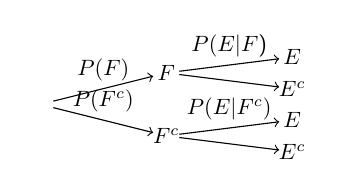
\begin{tikzpicture}[scale=0.8, every node/.style={transform shape}]
      \node[minimum size=4mm, inner sep=0] (O) at (0,1.25) {};
      \node[label=center:{$F$}, minimum size=4mm, inner sep=0] (F) at (2,1.75) {};
      \node[label=center:{$F^c$}, minimum size=4mm, inner sep=0] (Fc) at (2,0.75) {};
      \node[label=center:{$E$}, minimum size=4mm, inner sep=0] (FE) at (4,2) {};
      \node[label=center:{$E^c$}, minimum size=4mm, inner sep=0] (FEc) at (4,1.5) {};
      \node[label=center:{$E$}, minimum size=4mm, inner sep=0] (FcE) at (4,1) {};
      \node[label=center:{$E^c$}, minimum size=4mm, inner sep=0] (FcEc) at (4,0.5) {};
      \draw[->] (F) -- (FE) node[midway, above] {$P(E\vert F$)};
      \draw[->] (F) -- (FEc) node[midway, above] {};
      \draw[->] (Fc) -- (FcE) node[midway, above] {$P(E\vert F^c)$};
      \draw[->] (Fc) -- (FcEc) node[midway, above] {};
      \draw[->] (O) -- (F) node[midway, above] {$P(F)$};
      \draw[->] (O) -- (Fc) node[midway, above] {$P(F^c)$};
    \end{tikzpicture}
  \end{minipage}
  \begin{minipage}[c]{0.55\linewidth}
    $P(F \vert E) = \frac{P(EF)}{P(E)} = \frac{P(F) \cdot P(E \vert F)}{P(E)}$ \\
    $P(F^c \vert E) = \frac{P(EF^c)}{P(E)} = \frac{P(F^c) \cdot P(E \vert F^c)}{P(E)}$ 
  \end{minipage}

  \subsubsection{Total Probabililty}

  \textbf{theorem of total probability} - 
  Suppose $F_1, F_2, \dots, F_n$ are mutually exclusive events such that $\bigcup\limits^n_{i=1}F_i = S$, 
  then $P(E) = \sum\limits^n_{i=1}P(EF_i) = \sum\limits^n_{i=1}P(F_i)P(E\vert F_i)$

  \subsubsection{Bayes Theorem}

  \begin{align*}
    P(F_j \vert E) &= \frac{P(EF_j)}{P(E)} \\
                   &= \frac{P(F_j)P(E \vert F_j)}{\sum\limits^n_{i=1} P(F_i)P(E \vert F_i)}
  \end{align*}

  \textbf{application of bayes' theorem}

  \begin{tightcenter}
    $P(B_1 \mid A) = \frac{P(A \mid B_1) \cdot P(B_1)}{P(A \mid B_1) \cdot P(B_1) + P(A \mid B_2) \cdot P(B_2)}$
  \end{tightcenter}

  Let $A$ be the event that the person test positive for a disease.
  \\* $B_1$: the person actually has the disease.
  \\* $B_2$: the person does not have the disease.
  \begin{tightcenter}
    \begin{multicols}{2}
      true positives: $P(B_1\mid A)$
      \\ false positives: $P(A \mid B_2)$
      \\ false negatives: $P(\bar{A} \mid B_1)$
      \\ true negatives: $P(\bar{A} \mid B_2)$
    \end{multicols}
  \end{tightcenter}

  \subsection{Independent Events}

  \textbf{N1} - $E$ and $F$ are independent $\iff$
  \\* $P(EF) = P(E) \cdot P(F) \quad$ or $\quad P(E \vert F) = P(E)$

  \textbf{N2} - if $E$ and $F$ are independent, then $E$ and $F^c$ are independent.

  \textbf{N3} - if $E, F, G$ are independent, then $E$ will be independent of any event formed from $F$ and $G$. (e.g. $F\cup G$)


  \section{04. RANDOM VARIABLES}

  \subsection{Random Variables}

  \begin{itemize}
    \item \definition{random variable} a real-valued function defined on the sample space
    \item $X$ is a \definition[with parameter $p$ if]{Bernoulli r.v.} 
      \\* $p(x) = \begin{cases}
        p, &x=1, \text{ ('success')} \\
        1-p, &x=0\quad  \text{ ('failure')}
      \end{cases}$
  \end{itemize}










































\end{multicols*}

\begin{center}
  \begin{tabular}{ccc}
    \textbf{commutative} & $E \cup F = F \cup E$ & $E \cap F = F \cap E$ \\
    \textbf{associative} & $(E \cup F) \cup G = E \cup (F \cup G)$ &  $(E \cap F) \cap G = E \cap (F \cap G)$ \\
    \textbf{distributive} & $(E \cup F) \cap G = (E \cap F) \cup (F \cap G)$ & $(E \cap F) \cup G = (E \cup F) \cap (F \cup G)$ \\
    \textbf{DeMorgan's} & $(\bigcup\limits^n_{i=1} E_i)^c = \bigcap\limits^n_{i=1}E_i^c$ & $(\bigcap\limits^n_{i=1}E_i)^c = \bigcup\limits^n_{i=1}E_i^c$ \\
  \end{tabular}
\end{center}

\end{document}
